\section{Materials and Methods}

We first state our problem, then describe our data, showing all its characteristics. Then, we provide our hypothesis, define the setup, and perform the testing. Finally, we collect and perform data and regression analysis.

\subsection{Problem Statement}

As introduced in the first section of this paper, sorting is a fundamental concept and essential for solving other problems. The content of memory location can change unexpectedly, i.e., faults may happen at any time. Considering this, the main objective of this work is to design experiments to answer the following question: \textit{How are sorting algorithms affected by memory faults?}

\subsection{Variables}

For this experimental study, we assume that the dependent and independent variables are as shown in Table \ref{table-variables} below:

\begin{table}[H]
    \caption{Dependent and independent variables.}
    \begin{center}
    \begin{tabular}{|c|c|}
    \hline
    \multicolumn{2}{|c|}{\textbf{Variables}}\\
    \hline
    \textbf{\textit{Dependent}} & \textbf{\textit{Independent}} \\
    \hline
    Largest subarray size & Probability of failure \\
    Percentage of largest subarray size related to the original array & Array size \\
    Unordered elements size & Sorting algorithm \\
    Percentage of unordered elements size related to the original array & \\
    \hline
    \end{tabular}
    \label{table-variables}
    \end{center}
\end{table}

\subsection{Hypothesis}

We define a set of hypothesis to test and draw some conclusions. They are:

\setcounter{hyp}{-1}
\begin{hyp}[Test hypothesis] \label{hyp:a}There is no difference in memory faults between tested algorithms.\end{hyp}
\begin{hyp} \label{hyp:b}There are differences in memory faults between tested algorithms. \end{hyp}
\begin{hyp} \label{hyp:c} An algorithm is better than others considering all dependent variables. \end{hyp}

\begin{hyp} \label{hyp:d} ... \end{hyp}

\subsection{Experimental Setup}

To conduct the proposed study we get a set of files with the basic setup and instructions, that was composed by:
\begin{itemize}
    \item A file that contains a sequence of integers that are the input data;
    \item Four files, one for each os those algorithms: quicksort, bubblesort, insertion sort, and mergesort, that are used to sorting the input data;
    \item An output file with the sorted data.
\end{itemize}

The input file looks like follow:

\begin{verbbox}[\mbox{}]
0.01 100 9 48 37 6 26 7 24 44 17 50 48 30 49 33 22 13 42 29 39 13 19 13 9 28 
34 1 33 27 14 45 48 40 11 17 6 50 9 44 20 16 37 45 23 14 38 29 10 49 44 46 35
45 15 2 22 1 46 40 8 48 23 23 32 35 3 15 8 36 17 24 27 48 28 5 28 50 44 4 25 
6 9 1 11 44 26 50 44 12 7 20 30 20 37 20 6 8 13 15 20 49
\end{verbbox}

\begin{figure}[H]
    \centering
    \fbox{
    \theverbbox
    }
    \caption{Example of input file.}
    \label{fig-input-file-example}
\end{figure}

The input data shown in the Figure \ref{fig-input-file-example} is divided as follows:

\begin{itemize}
    \item \textit{Probability of Failure}: the first number of the sequence (\texttt{0.01}) is the probability of memory failure when sorting;
    \item \textit{Sequence size}: the second number (\texttt{100}) means the size of the integers sequence used by sorting;
    \item \textit{Sequence}: the rest of the numbers indicates the sequence itself.
\end{itemize}

We run 1000 times each algorithm with each file listed in Table \ref{table-input-data} below. We chose this number of executions to reduce possible noise in the generated data. Table \ref{table-input-data} shows 9 different input files with its sequence sizes and probabilities of failure. Plus, the number of executions and each sorting algorithm.

For example, Input A showed in that table with its characteristics was executed 1000 times for each algorithm -  bubblesort, quicksort, mergesort, and insertion sort - totalizing 4000 executions.

\begin{table}[H]
    \caption{Generated input data.}
    \begin{center}
    \begin{tabular}{|c|c|c|c|c|}
    \hline
    \textbf{Input} & \textbf{Sequence Size} & \textbf{Probability of Failure} & \textbf{Executions} & \textbf{Algorithm} \\ 
    \hline
    \multirow{4}{*}{Input A} & \multirow{4}{*}{100} & \multirow{4}{*}{1\%} & \multirow{4}{*}{1000} & Bubblesort \\ 
    & & & & Quicksort \\
    & & & & Mergesort \\
    & & & & Insertion Sort \\
    \hline
    \multirow{4}{*}{Input B} & \multirow{4}{*}{100} & \multirow{4}{*}{2\%} & \multirow{4}{*}{1000} & Bubblesort \\ 
    & & & & Quicksort \\
    & & & & Mergesort \\
    & & & & Insertion Sort \\
    \hline
    \multirow{4}{*}{Input C} & \multirow{4}{*}{100} & \multirow{4}{*}{5\%} & \multirow{4}{*}{1000} & Bubblesort \\ 
    & & & & Quicksort \\
    & & & & Mergesort \\
    & & & & Insertion Sort \\
    \hline
    \multirow{4}{*}{Input D} & \multirow{4}{*}{1000} & \multirow{4}{*}{1\%} & \multirow{4}{*}{1000} & Bubblesort \\ 
    & & & & Quicksort \\
    & & & & Mergesort \\
    & & & & Insertion Sort \\
    \hline
    \multirow{4}{*}{Input E} & \multirow{4}{*}{1000} & \multirow{4}{*}{2\%} & \multirow{4}{*}{1000} & Bubblesort \\ 
    & & & & Quicksort \\
    & & & & Mergesort \\
    & & & & Insertion Sort \\
    \hline
    \multirow{4}{*}{Input F} & \multirow{4}{*}{1000} & \multirow{4}{*}{5\%} & \multirow{4}{*}{1000} & Bubblesort \\ 
    & & & & Quicksort \\
    & & & & Mergesort \\
    & & & & Insertion Sort \\
    \hline
    \multirow{4}{*}{Input G} & \multirow{4}{*}{10000} & \multirow{4}{*}{1\%} & \multirow{4}{*}{1000} & Bubblesort \\ 
    & & & & Quicksort \\
    & & & & Mergesort \\
    & & & & Insertion Sort \\
    \hline
    \multirow{4}{*}{Input H} & \multirow{4}{*}{10000} & \multirow{4}{*}{2\%} & \multirow{4}{*}{1000} & Bubblesort \\ 
    & & & & Quicksort \\
    & & & & Mergesort \\
    & & & & Insertion Sort \\
    \hline
    \multirow{4}{*}{Input I} & \multirow{4}{*}{10000} & \multirow{4}{*}{5\%} & \multirow{4}{*}{1000} & Bubblesort \\ 
    & & & & Quicksort \\
    & & & & Mergesort \\
    & & & & Insertion Sort \\
    \hline
    \end{tabular}
    \label{table-input-data}
    \end{center}
\end{table}

Each execution generates an output file. Then, we generate 4000 outputs for each combination of sequence size, and the probability of failure, totalizing 36000 files. Figure \ref{fig-output-file-example} shows an output file.

\begin{verbbox}[\mbox{}]
[1]  9 48 37 6 26 7 24 44 17 50 48 30 49 33 22 13 42 29 39 13 19 13 9 28 34 1
33 27 14 45 48 40 11 17 6 50 9 44 20 16 37 45 23 14 38 29 10 49 44 46 35 45  
15 2 22 1 46 40 8 48 23 23 32 35 3 15 8 36 17 24 27 48 28 5 28 50 44 4 25 6 9
1 11 44 26 50 44 12 7 20 30 20 37 20 6 8 13 15 20 49
[2]  1 1 1 2 3 4 5 6 6 6 6 7 7 8 8 8 9 9 9 9 10 11 11 12 13 13 13 13 14 14 15 
15 15 16 17 17 17 19 20 20 20 20 22 22 23 23 23 24 24 25 26 26 27 27 28 28 28 
29 29 30 30 32 33 33 34 35 35 36 37 37 37 38 39 40 40 42 44 44 44 44 44 44 20 
45 45 45 46 46 48 48 48 48 48 49 49 50 49 50 50 50
[3]  1 1 1 2 3 4 5 6 6 6 6 7 7 8 8 8 9 9 9 9 10 11 11 12 13 13 13 13 14 14 15 
15 15 16 17 17 17 19 20 20 20 20 20 22 22 23 23 23 24 24 25 26 26 27 27 28 28 
28 29 29 30 30 32 33 33 34 35 35 36 37 37 37 38 39 40 40 42 44 44 44 44 44 44 
45 45 45 46 46 48 48 48 48 48 49 49 49 50 50 50 50
[4]  82
\end{verbbox}
    
\begin{figure}[H]
    \centering
    \fbox{
    \theverbbox
    }
    \caption{Example of output file.}
    \label{fig-output-file-example}
\end{figure}

The output file gives four essential data, as enumerated below:
\begin{itemize}
    \item \textit{[1]}: the original sequence of integers contained in the input file;
    \item \textit{[2]}: the sequence processed by the sorting algorithm under the memory fault model;
    \item \textit{[3]}: the sequence sorted correctlty;
    \item \textit{[4]}: the size of the largest sorted subsequence in [2]. This number can be interpreted as the quality of sorting. As higher, most successful was the sorting operation.
\end{itemize}

\subsection{Development}

We develop Python scripts to generate our dataset. First, we generate all input files through a given script called \textit{gen.py}. This script considers sequence size and the probability of failure to create a sequence of integers. Were produced nine input files like Figure \ref{fig-input-file-example}, combining the sequence size and probability of failure listed in Table \ref{table-input-data}.

After that, we developed a script called \textit{main\_execution.py} that is responsible for creating output files based on the input files exposed before. At this time, for every input showed in Table \ref{table-input-data} we ran 1000 times to minimize any deviation on the quality of sorting indicator (line \textit{[4]} on Figure \ref{fig-output-file-example}).

As said before, after the execution of this algorithm, 4000 outputs for each combination of sequence size, and the probability of failure, totalizing 36000 files.

\textcolor{red}{To be continued...}

\subsection{Data Analysis}

In this section, we describe our data and the statistic tests used to test the hypothesis showed before.

\subsubsection{Exploratory Data Analysis (EDA)}

Based on the output files generated before, our starting point was to test if the dataset had a normal distribution. To achieve this, we use Shapiro-Wilk normality test. After we run these tests, only the distribution related to the dependent variable \textit{unordered elements size} was considered normal. Figure \ref{fig-distribution-graph} shows an example of this distribution. In these graphs, the red vertical line means the mean, and the blue vertical line means the median. The distributions were normal in all combinations of independent variables for dependent variable \textit{unordered elements size}.

\begin{figure}[H]
    \centering
     \begin{subfigure}{.5\textwidth}
     \centering
     \frame{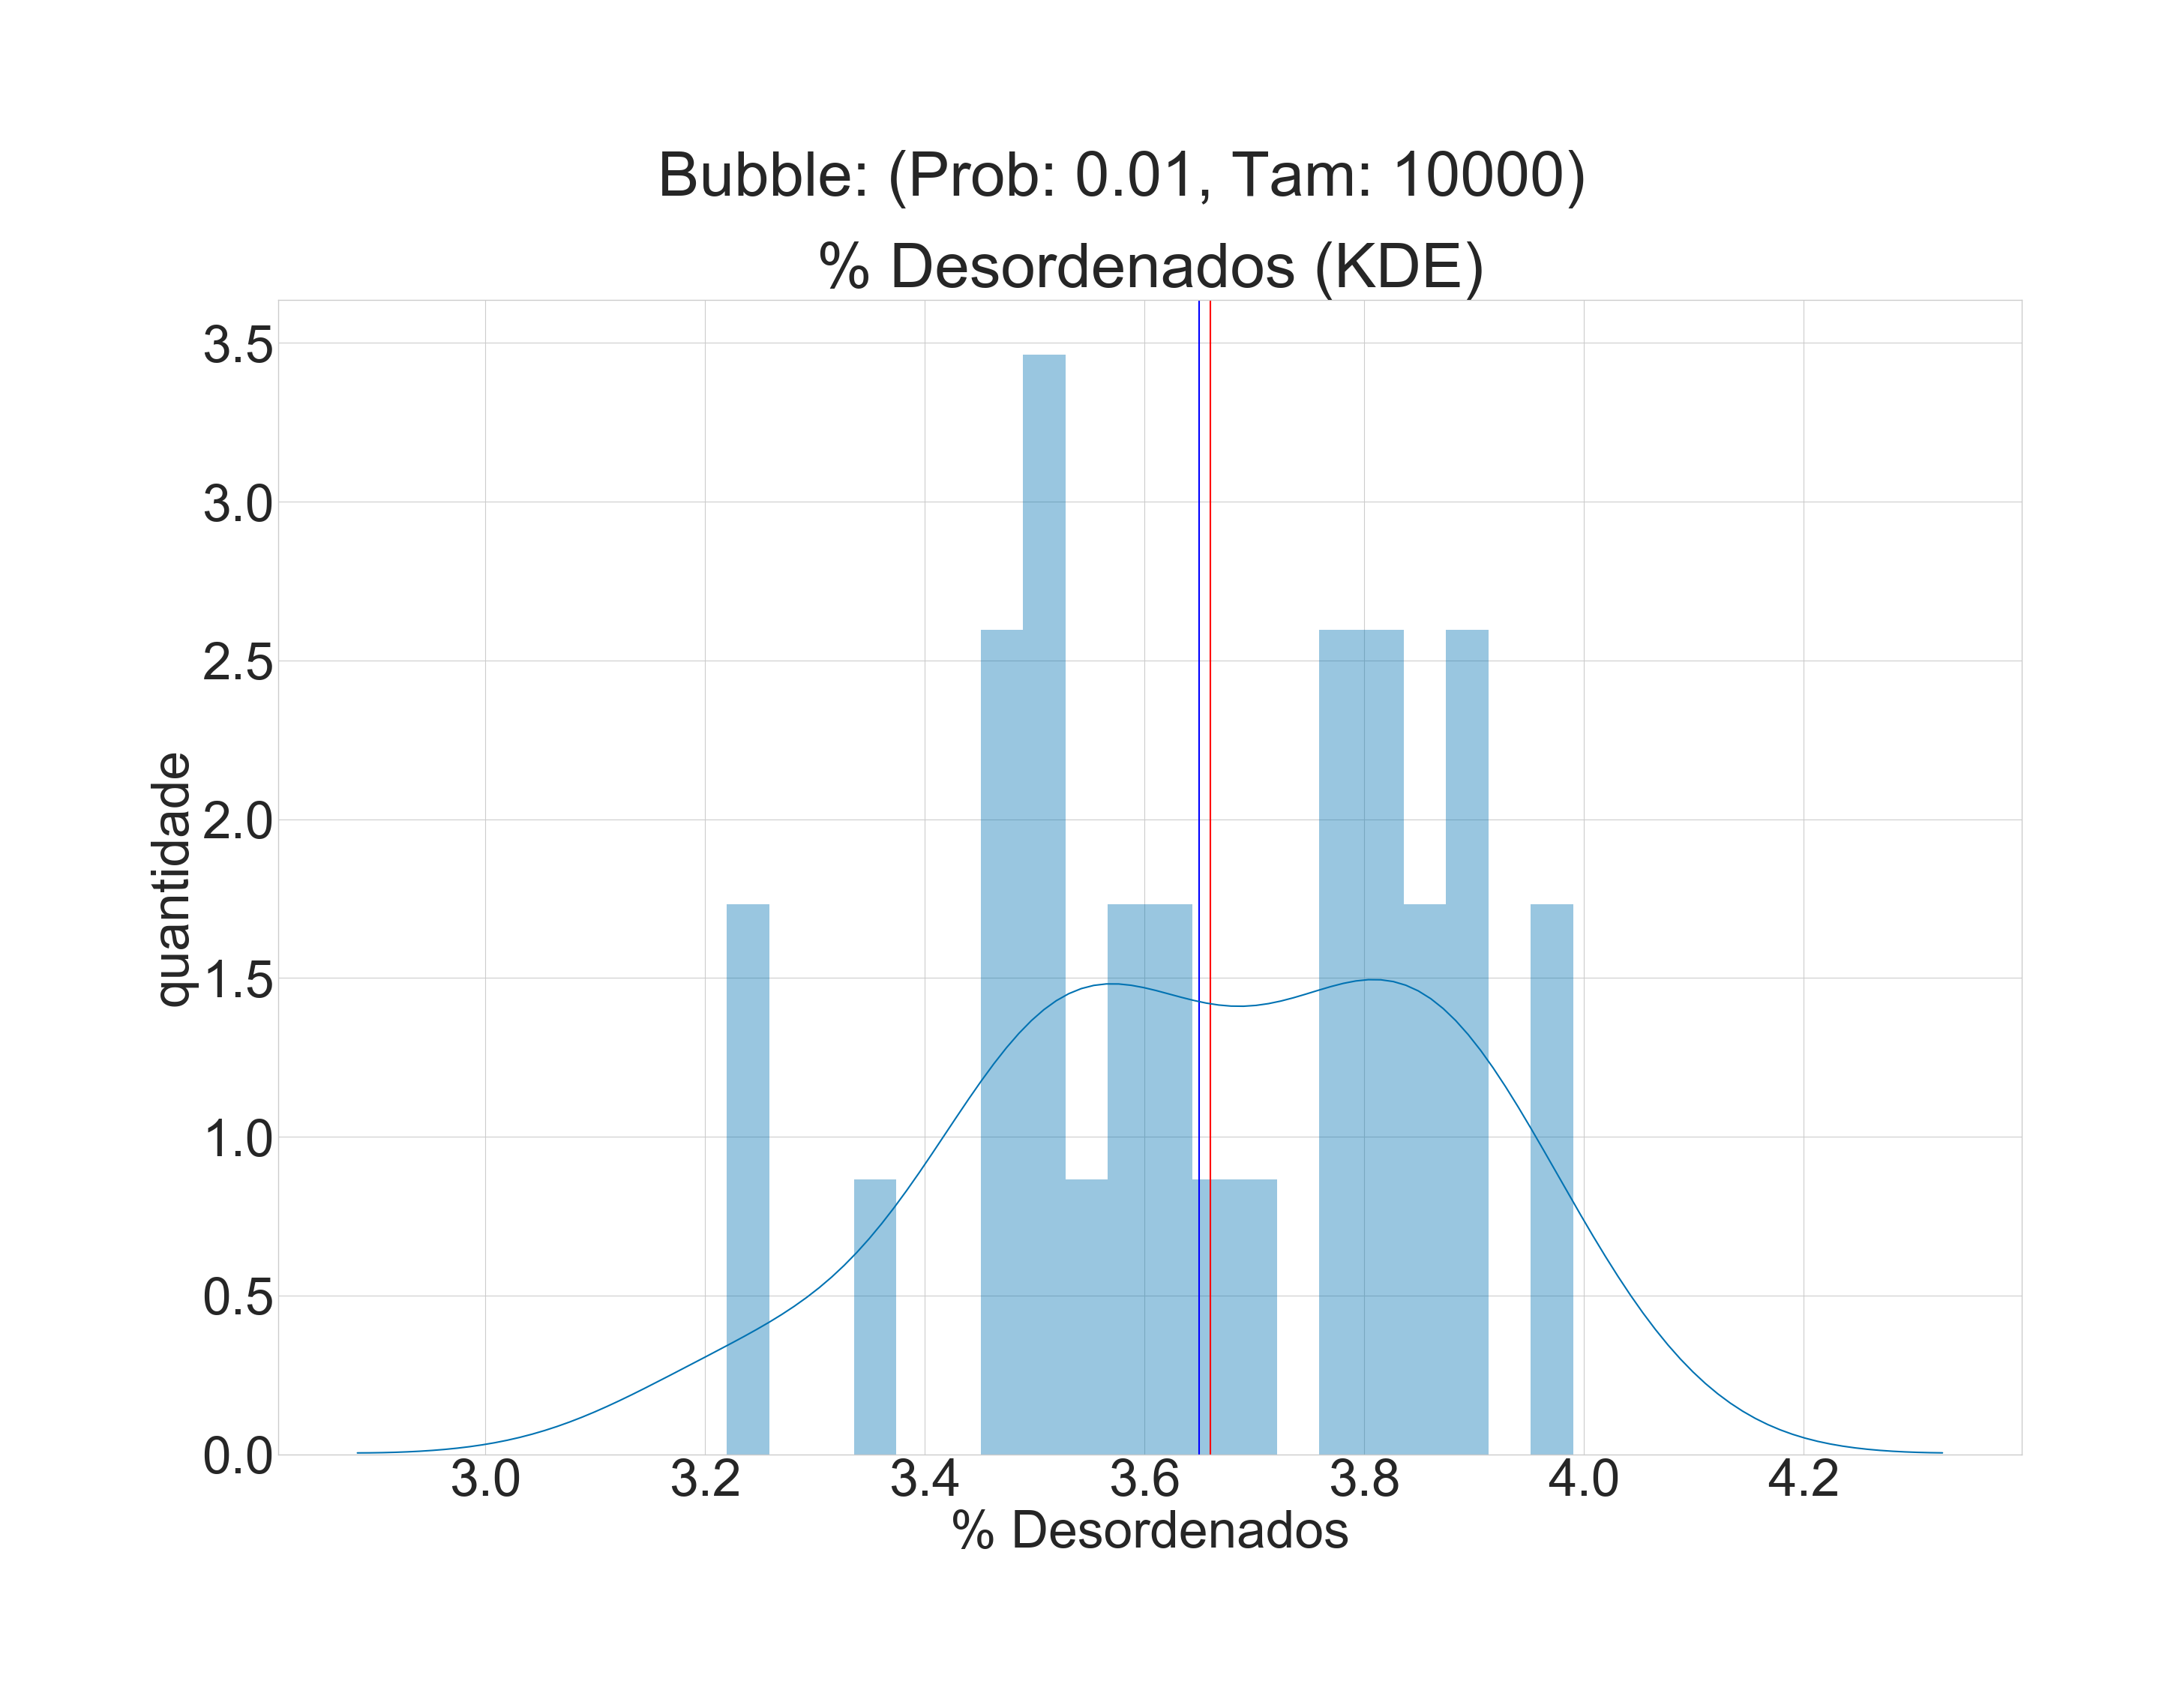
\includegraphics[scale=0.12]{figures/0_01_10000_Bubble_distribution_graph}}
     \textsf{\caption[Distribution Graph for bubblesort.]{Distribution Graph for bubblesort.\label{fig-dist-bubble-001-100}}}
     \end{subfigure}%
     \begin{subfigure}{.5\textwidth}
     \centering
     \frame{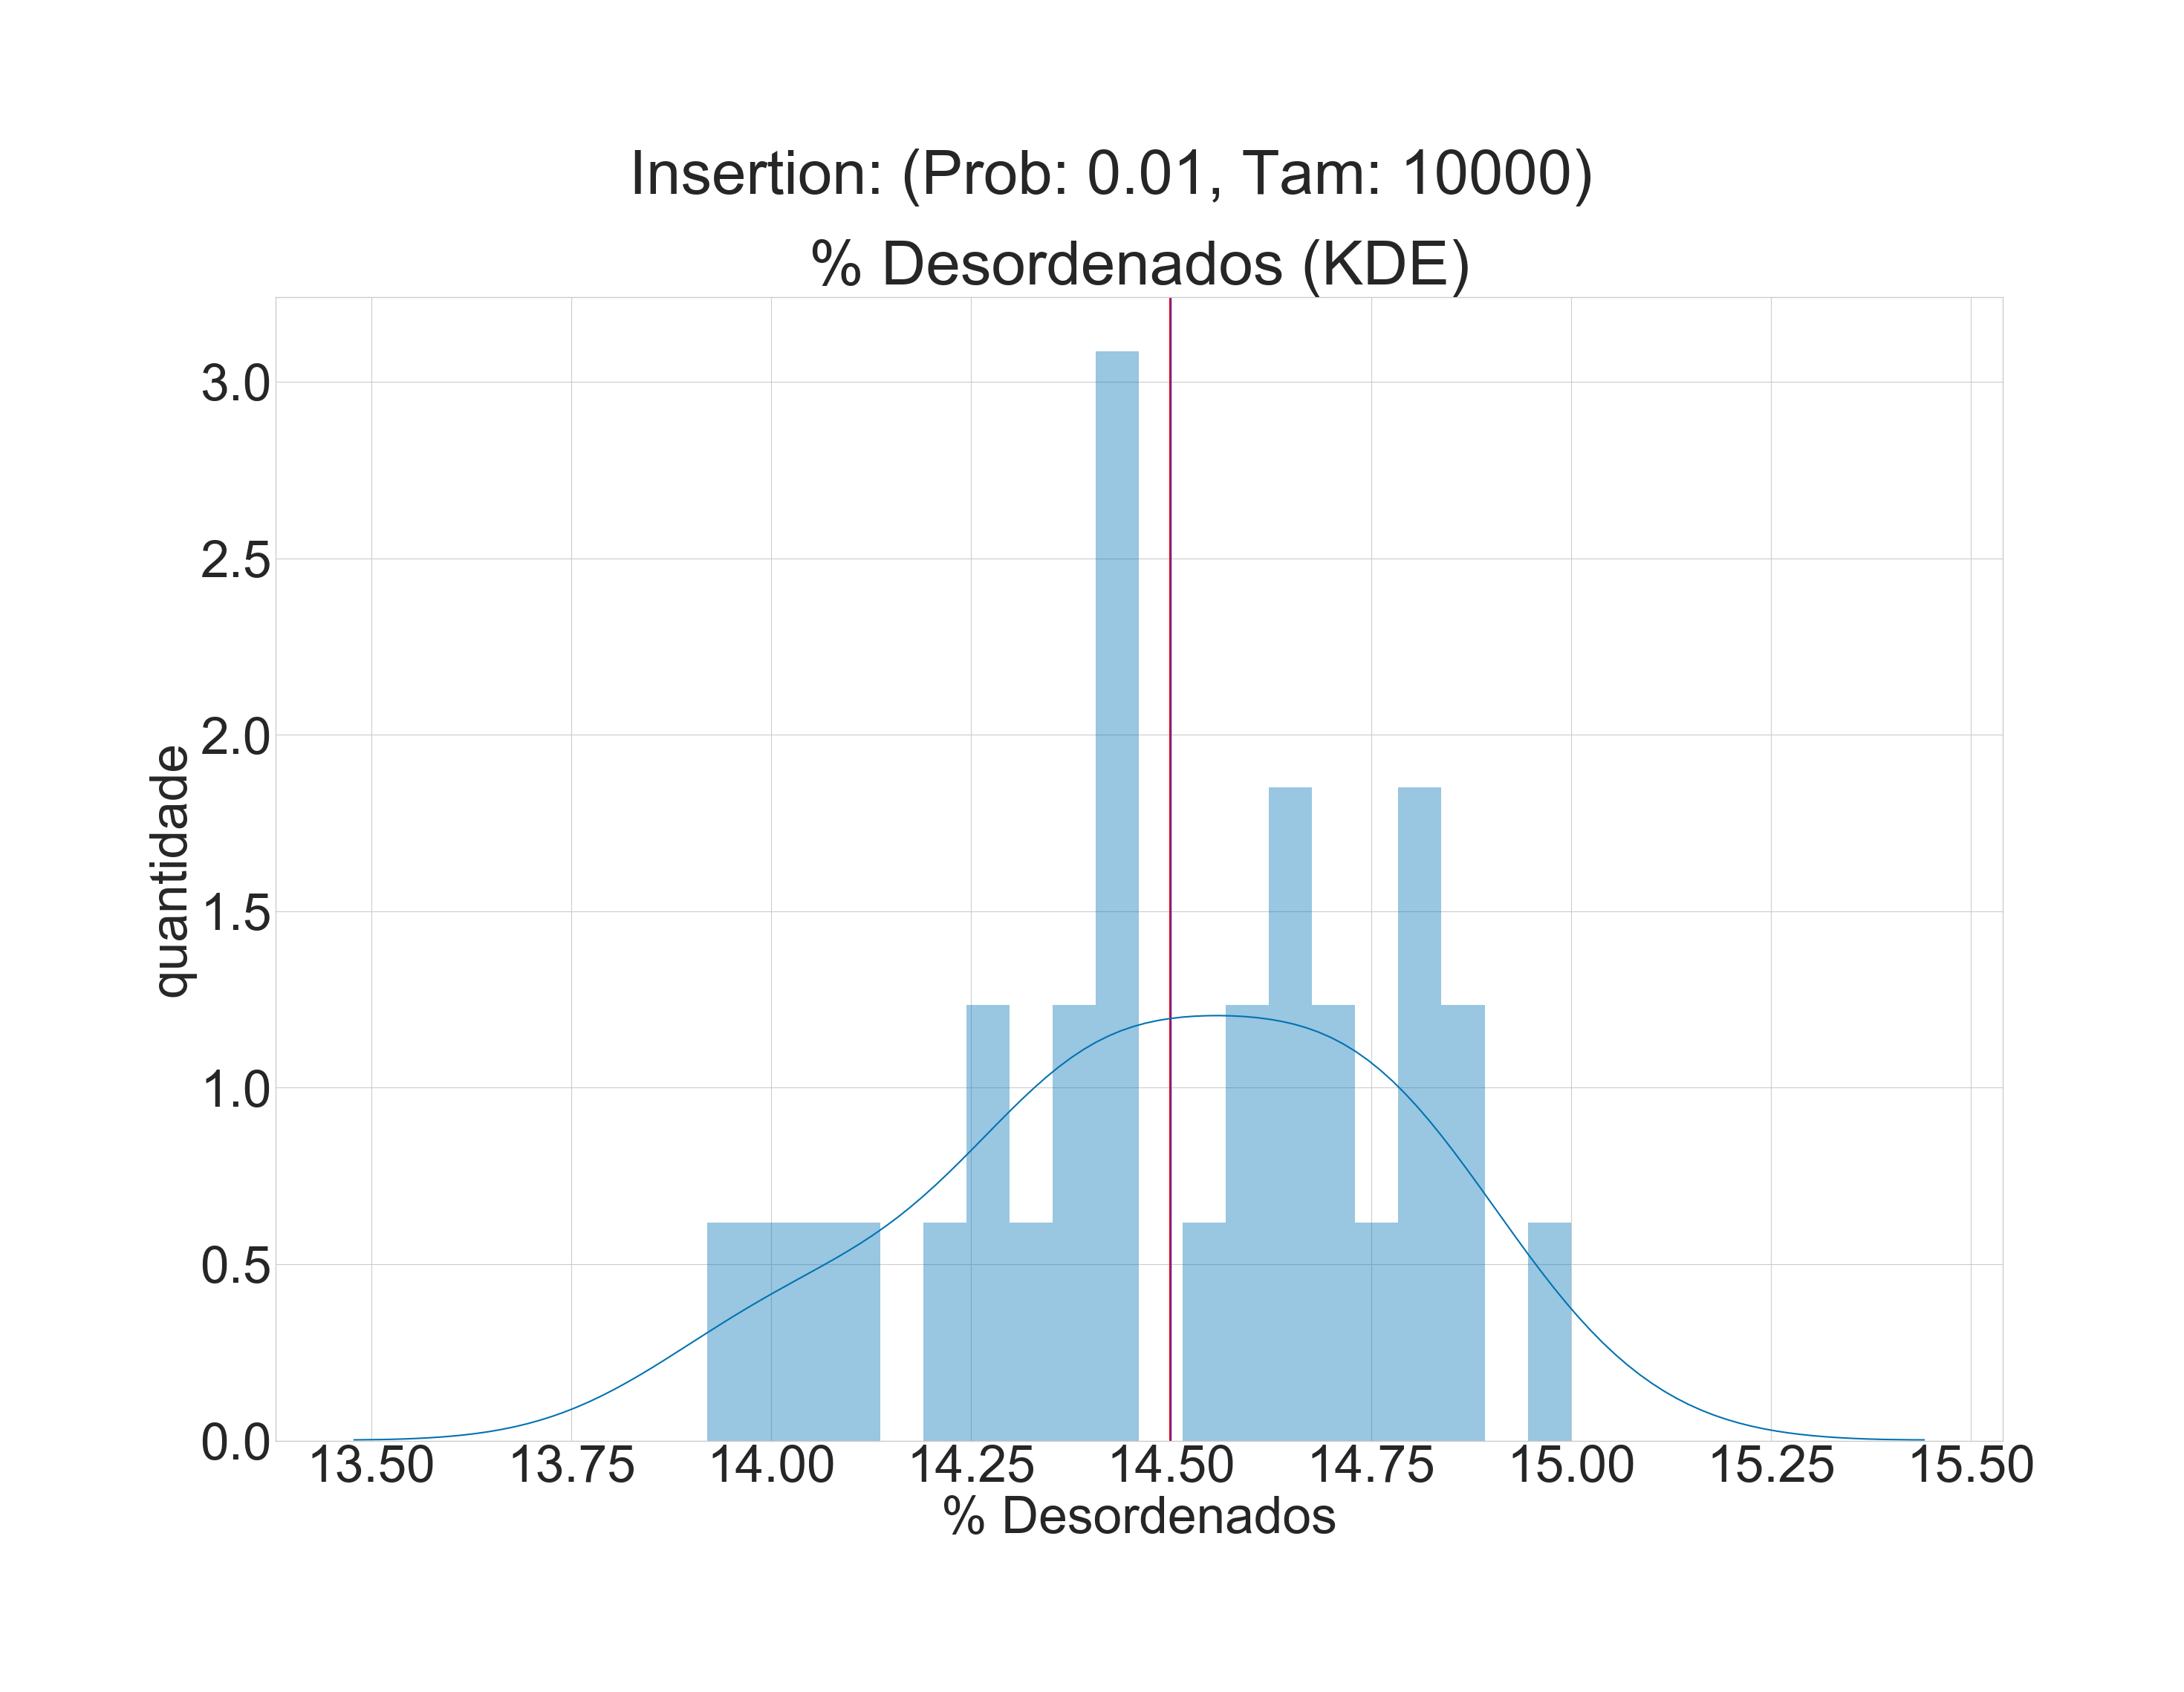
\includegraphics[scale=0.12]{figures/0_01_10000_Insertion_distribution_graph.png}}
     \textsf{\caption[Distribution Graph for insertion sort.]{Distribution Graph for insertion sort.\label{fig-dist-insertion-001-100}}}
     \end{subfigure}
     \begin{subfigure}{.5\textwidth}
     \centering
     \frame{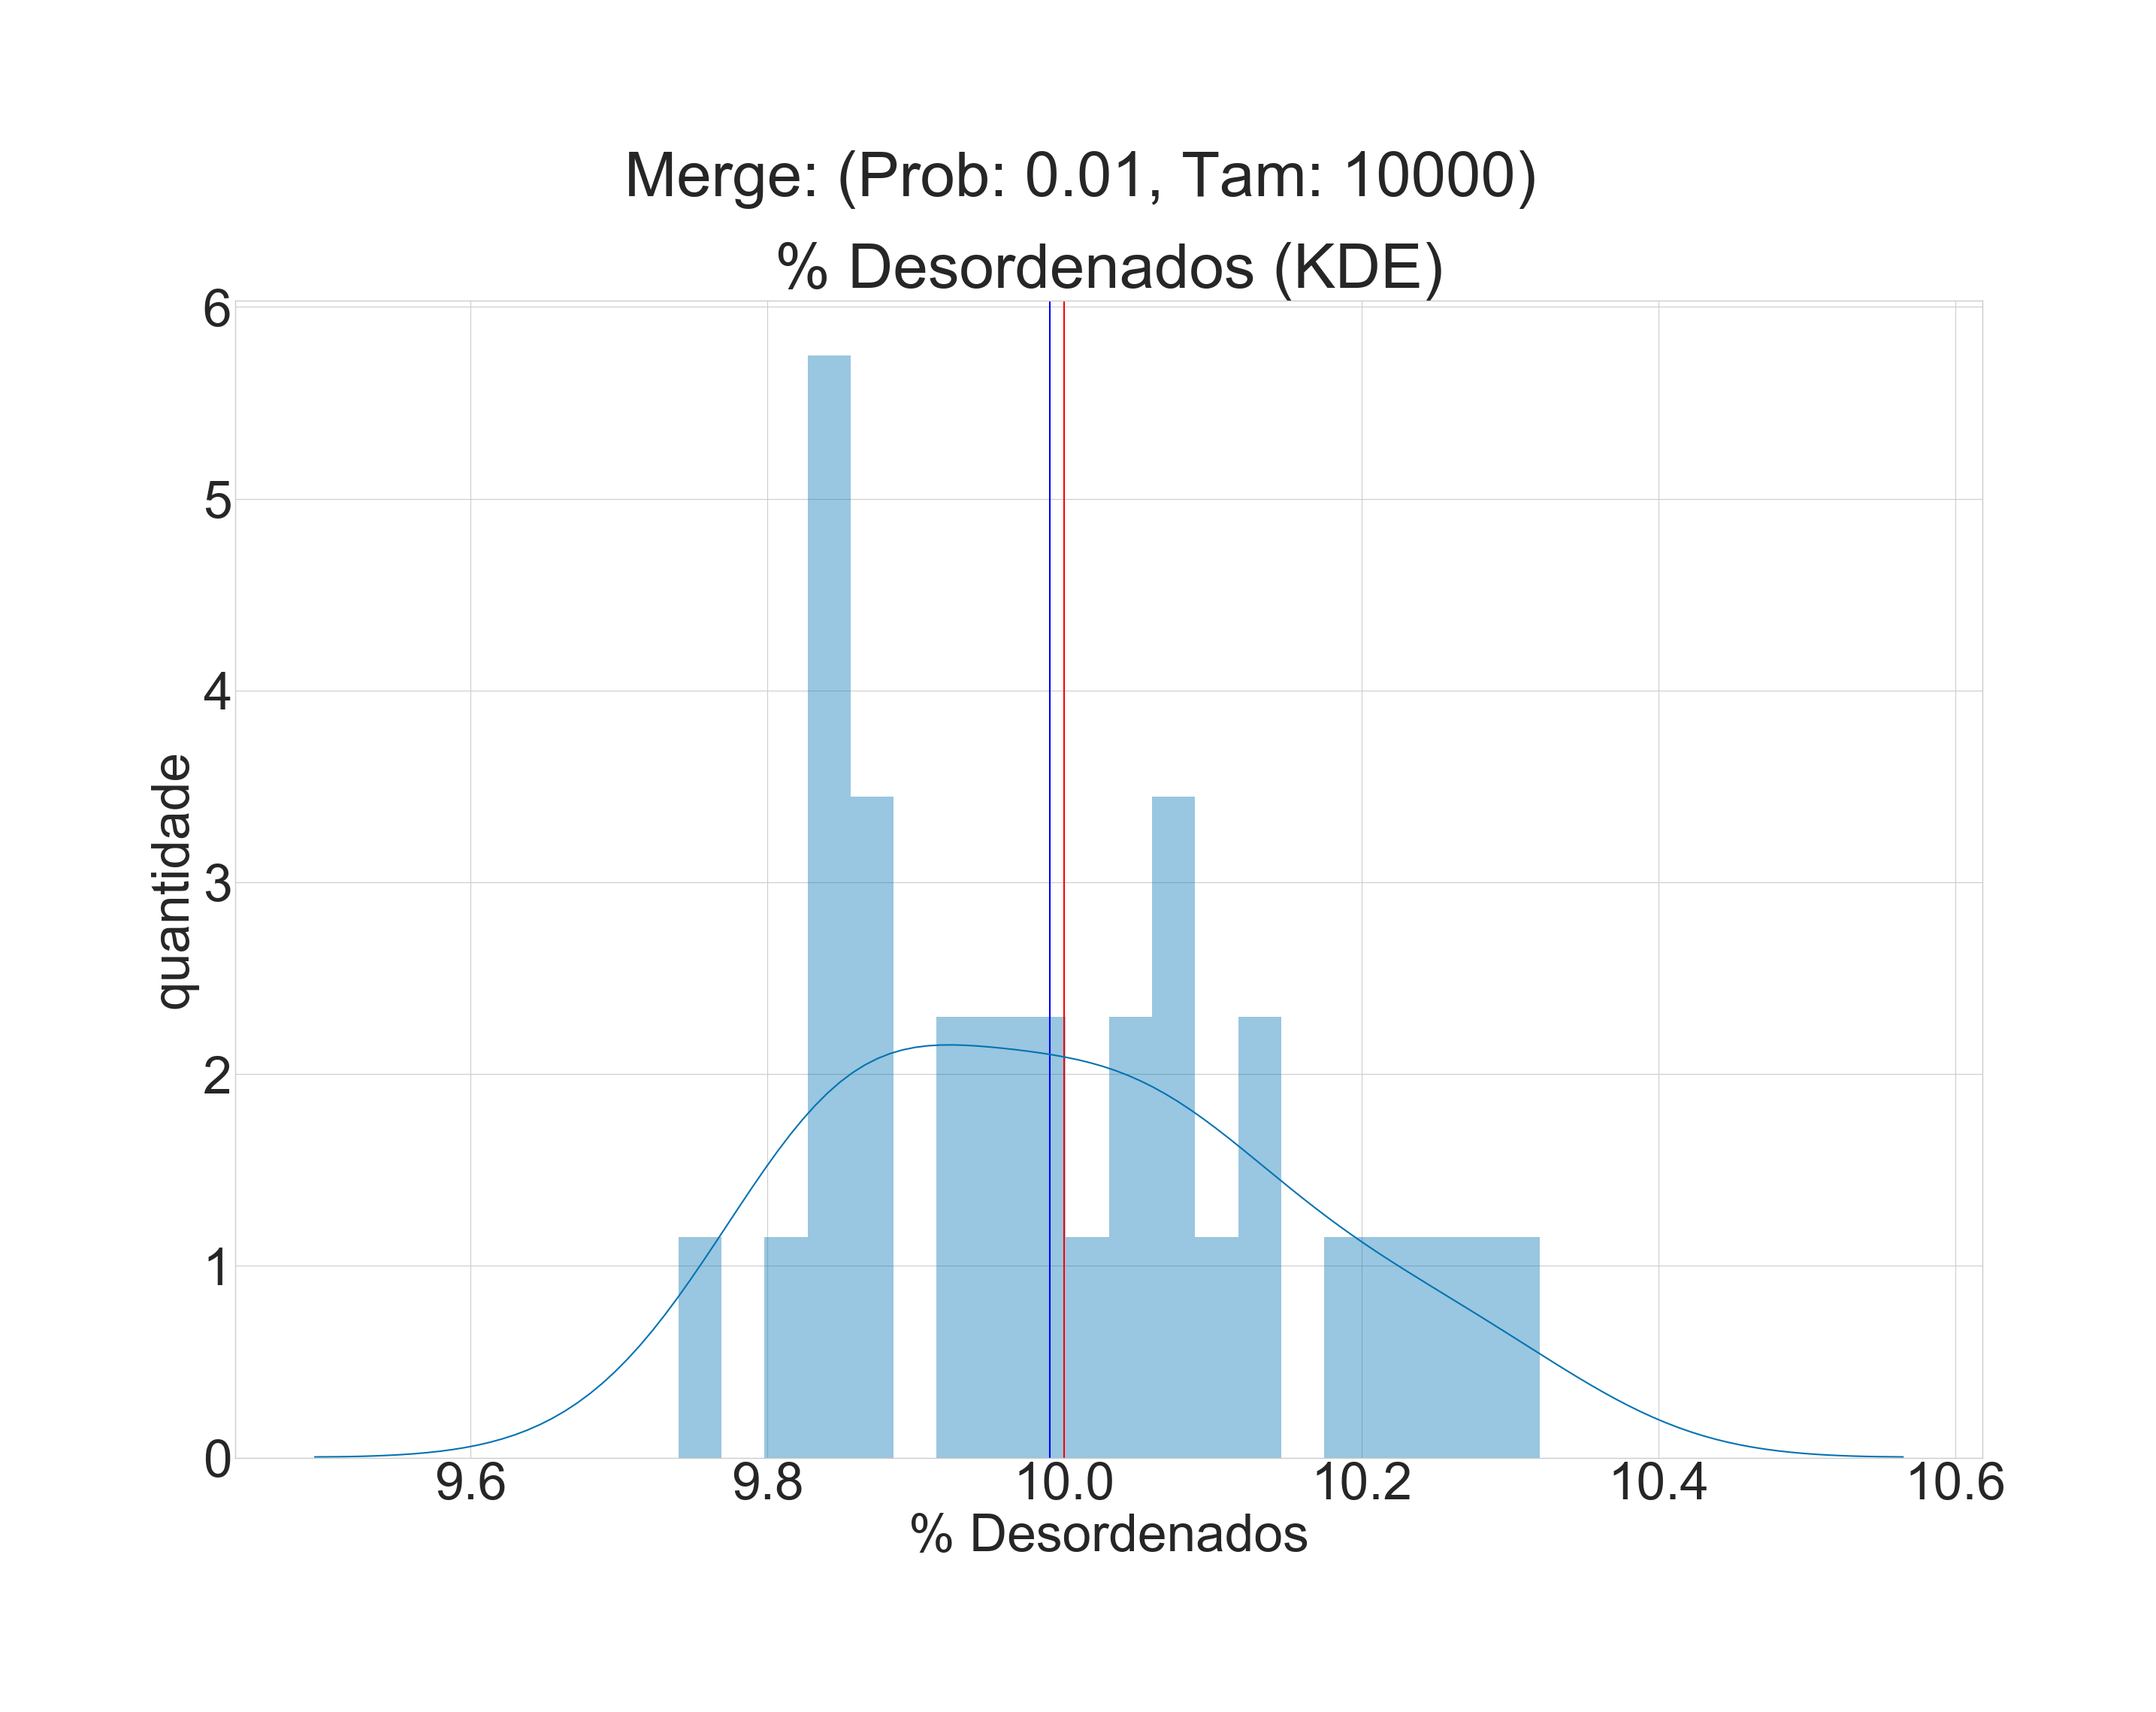
\includegraphics[scale=0.12]{figures/0_01_10000_Merge_distribution_graph.png}}
     \textsf{\caption[Distribution Graph for mergesort.]{Distribution Graph for mergesort.\label{fig-dist-merge-001-100}}}
     \end{subfigure}%
     \begin{subfigure}{.5\textwidth}
     \centering
     \frame{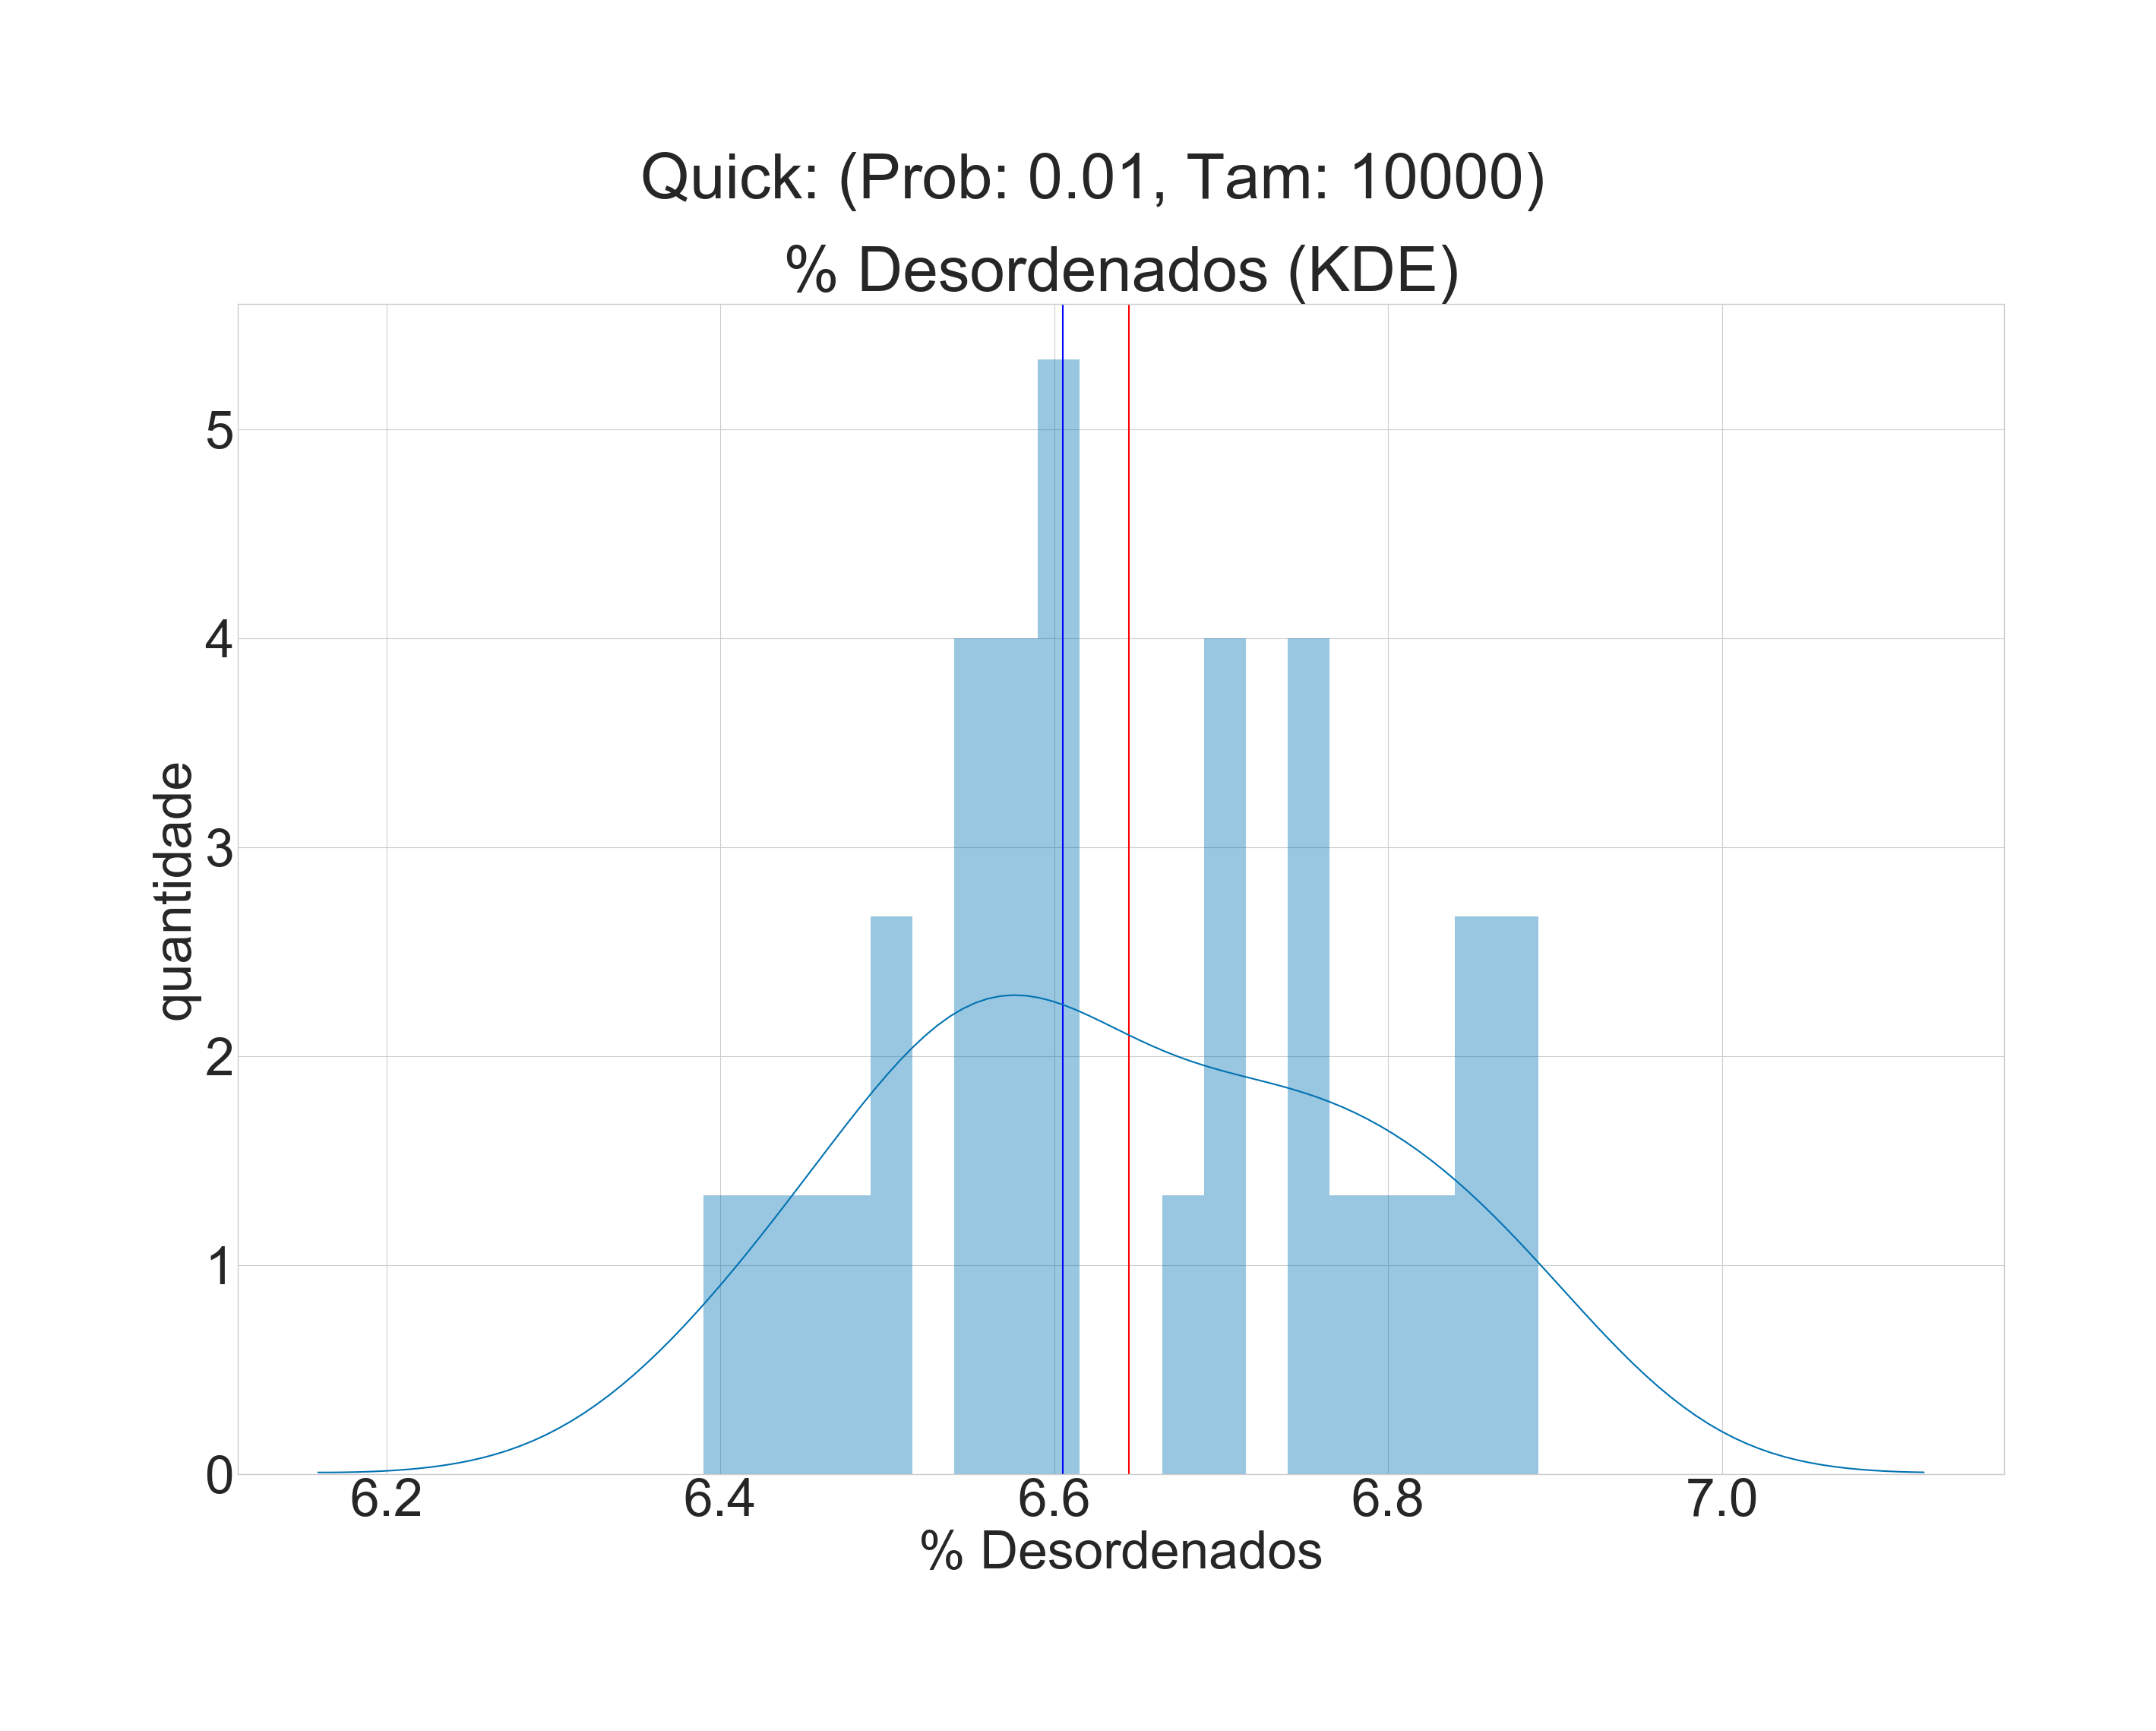
\includegraphics[scale=0.12]{figures/0_01_10000_Quick_distribution_graph.png}}
     \textsf{\caption[Distribution Graph for quicksort.]{Distribution Graph for quicksort.\label{fig-dist-quick-001-100}}}
     \end{subfigure}
     \caption{Distribution graph for a probability failure of 1\% and a sequence size of 10000.}
    \label{fig-distribution-graph}
\end{figure}

Q-Q plot shows that how much more blue points close to the red line, most normal is the distribution. Figure \ref{fig-qqplot} below presents this graph for a probability failure of 1\% and a sequence size of 10000 for considered sorting algorithms.

\begin{figure}[H]
    \centering
    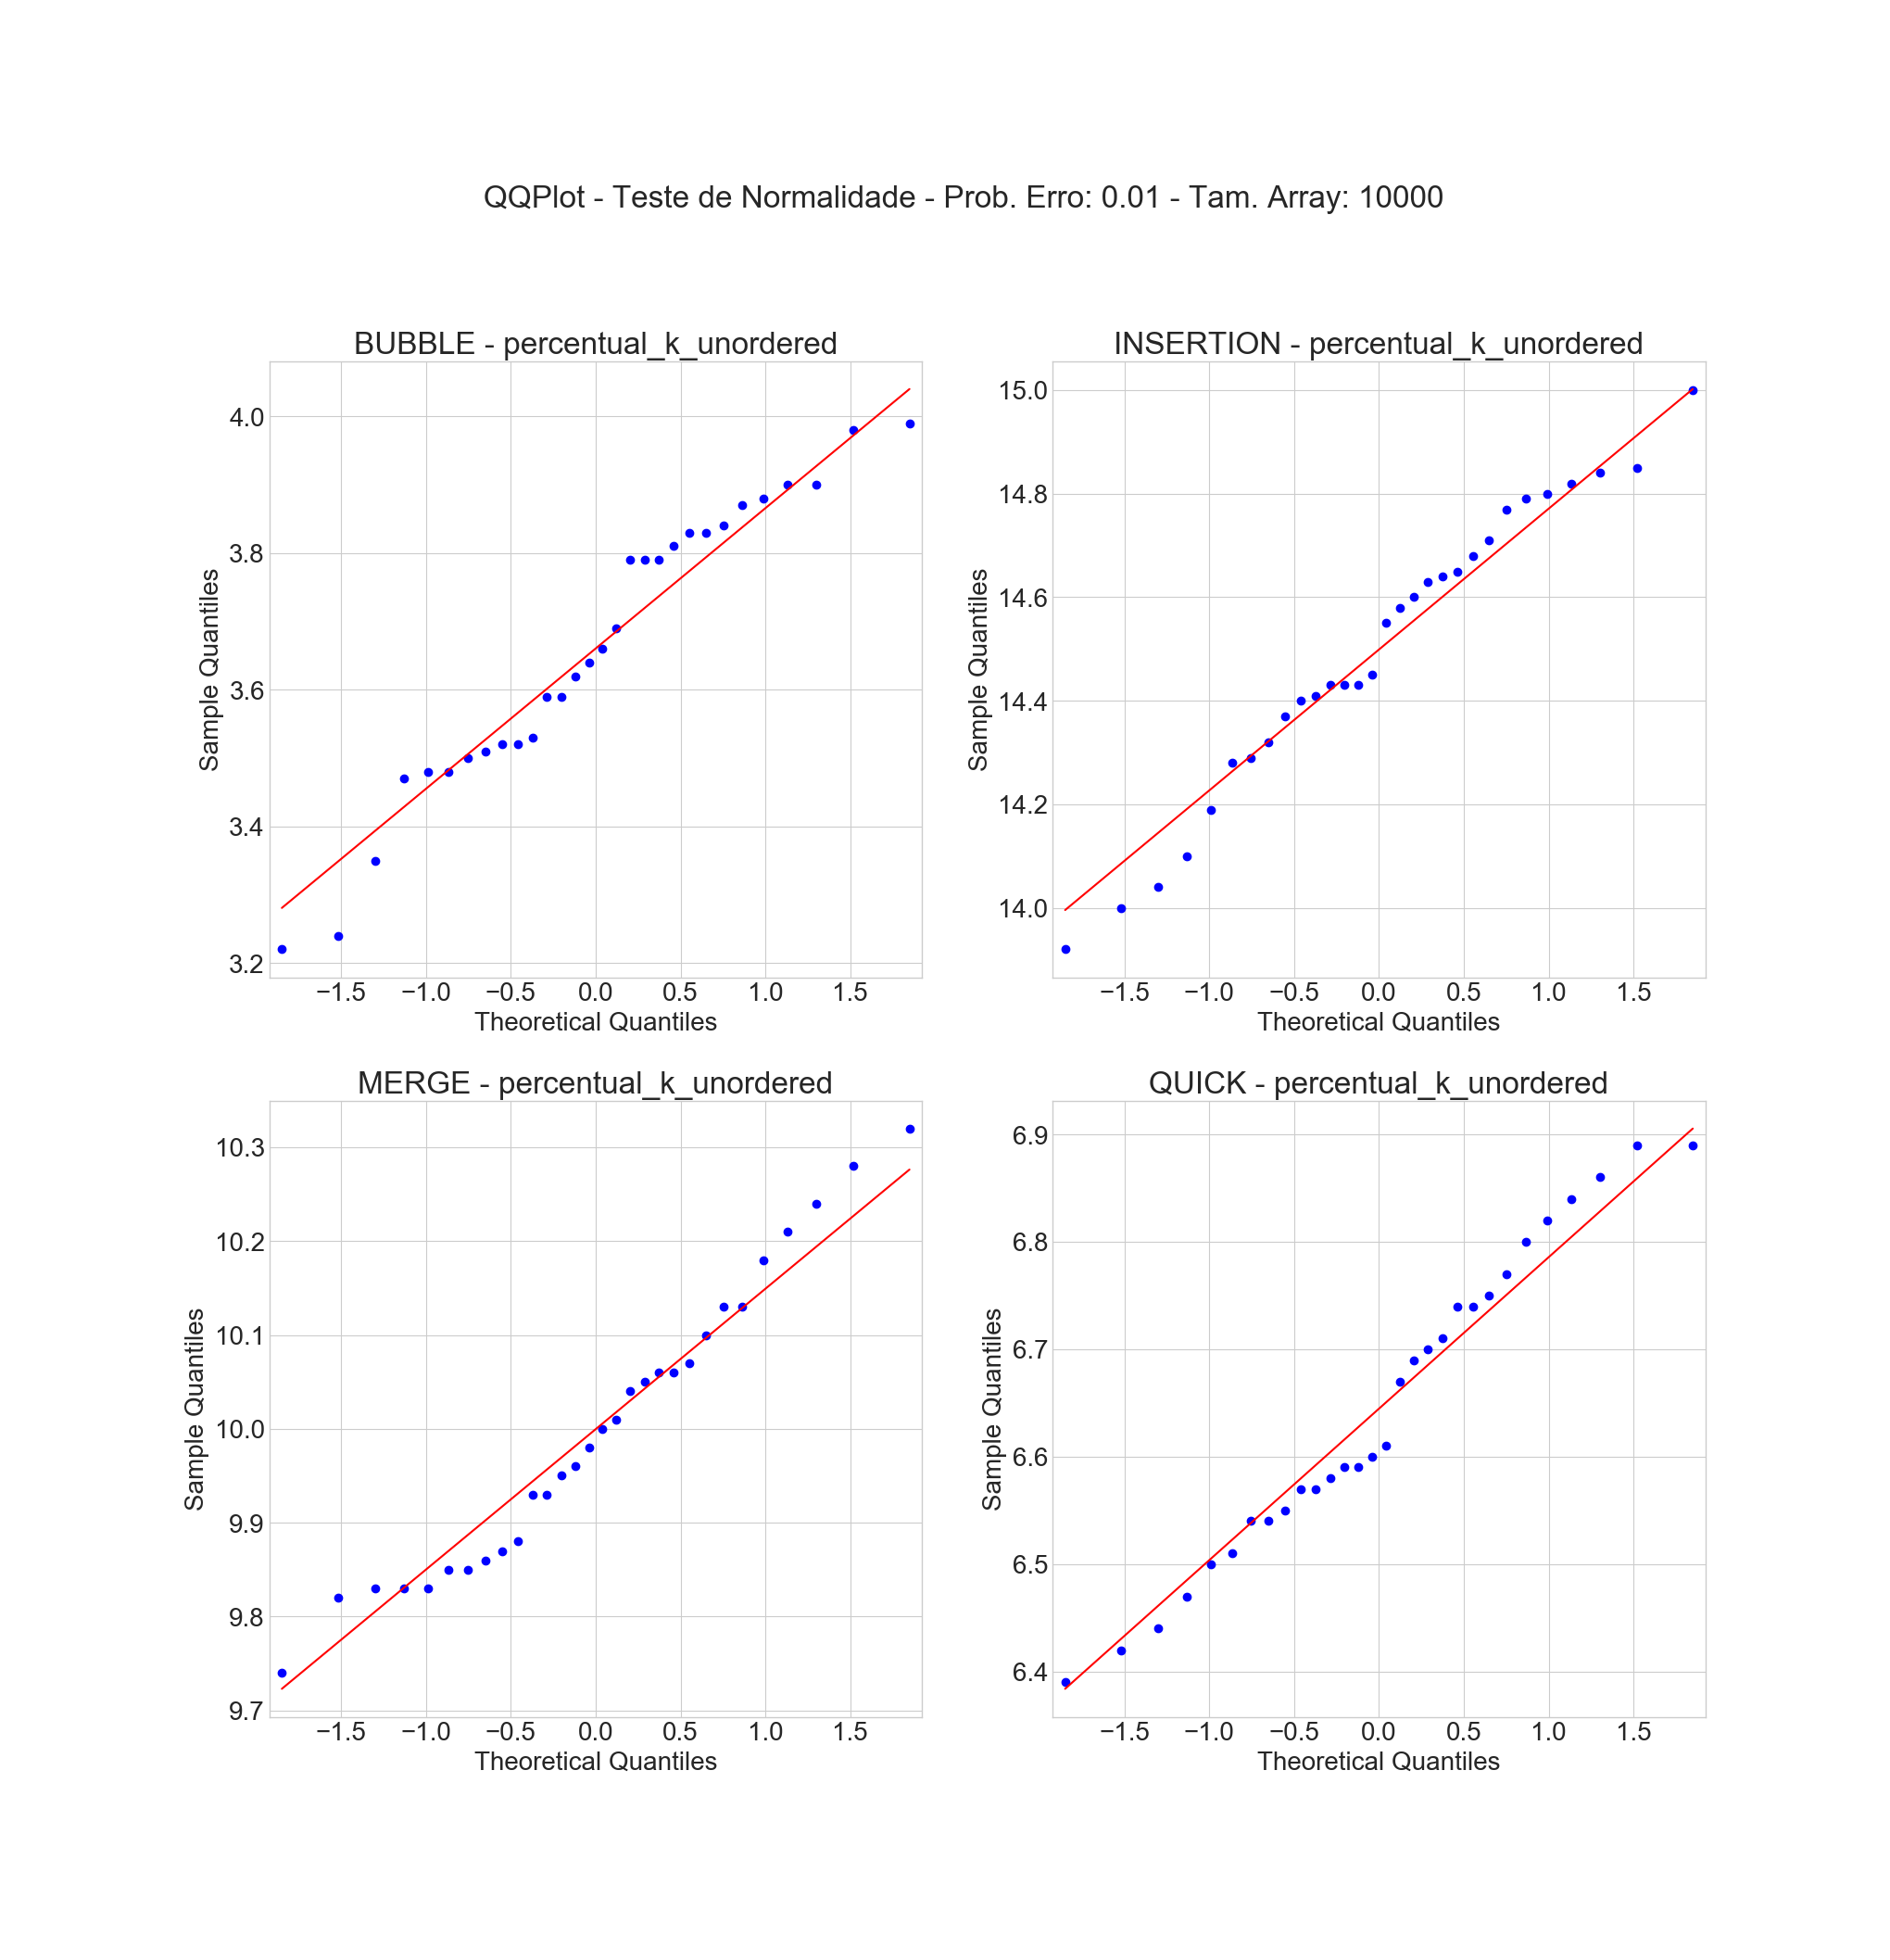
\includegraphics[scale=0.37]{figures/anova_prob_0_01_tam_10000_DESORDENADOS_PERCENTUAL.png}
    \textsf{\caption[Q-Q plot showing normal distribution for a probability failure of 1\% and a sequence size of 10000.]{Q-Q plot showing normal distribution for a probability failure of 1\% and a sequence size of 10000.\label{fig-qqplot}}}
 \end{figure}

\subsection{Conclusions}

